%%
%% This is file `sample-sigplan.tex',
%% generated with the docstrip utility.
%%
%% The original source files were:
%%
%% samples.dtx  (with options: `sigplan')
%%
%% IMPORTANT NOTICE:
%%
%% For the copyright see the source file.
%%
%% Any modified versions of this file must be renamed
%% with new filenames distinct from sample-sigplan.tex.
%%
%% For distribution of the original source see the terms
%% for copying and modification in the file samples.dtx.
%%
%% This generated file may be distributed as long as the
%% original source files, as listed above, are part of the
%% same distribution. (The sources need not necessarily be
%% in the same archive or directory.)
%%
%%
%% Commands for TeXCount
%TC:macro \cite [option:text,text]
%TC:macro \citep [option:text,text]
%TC:macro \citet [option:text,text]
%TC:envir table 0 1
%TC:envir table* 0 1
%TC:envir tabular [ignore] word
%TC:envir displaymath 0 word
%TC:envir math 0 word
%TC:envir comment 0 0
%%
%%
%% The first command in your LaTeX source must be the \documentclass command.
%%\documentclass[sigplan,nonacm]{acmart}
\documentclass[sigplan,screen,nonacm]{acmart}\settopmatter{printfolios=true,printccs=false,printacmref=false}
\graphicspath{{figure/}}
%%
%% \BibTeX command to typeset BibTeX logo in the docs
\AtBeginDocument{%
	\providecommand\BibTeX{{%
			\normalfont B\kern-0.5em{\scshape i\kern-0.25em b}\kern-0.8em\TeX}}}

%% Rights management information.  This information is sent to you
%% when you complete the rights form.  These commands have SAMPLE
%% values in them; it is your responsibility as an author to replace
%% the commands and values with those provided to you when you
%% complete the rights form.
\setcopyright{none}

%%\copyrightyear{2018}
%%\acmYear{2018}
%%\acmDOI{10.1145/1122445.1122456}

%% These commands are for a PROCEEDINGS abstract or paper.
%%\acmConference[Woodstock '18]{Woodstock '18: ACM Symposium%% on Neural
%%  Gaze Detection}{June 03--05, 2018}{Woodstock, NY}
%%\acmBooktitle{Woodstock '18: ACM Symposium on Neural Gaze Detection,
%%  June 03--05, 2018, Woodstock, NY}
%%\acmPrice{15.00}
%%\acmISBN{978-1-4503-XXXX-X/18/06}


%%
%% Submission ID.
%% Use this when submitting an article to a sponsored event. You'll
%% receive a unique submission ID from the organizers
%% of the event, and this ID should be used as the parameter to this command.
%%\acmSubmissionID{123-A56-BU3}

%%
%% The majority of ACM publications use numbered citations and
%% references.  The command \citestyle{authoryear} switches to the
%% "author year" style.
%%
%% If you are preparing content for an event
%% sponsored by ACM SIGGRAPH, you must use the "author year" style of
%% citations and references.
%% Uncommenting
%% the next command will enable that style.
%%\citestyle{acmauthoryear}

%%
%% end of the preamble, start of the body of the document source.
\begin{document}
\sloppy

%%
%% The "title" command has an optional parameter,
%% allowing the author to define a "short title" to be used in page headers.
\title{A brief study of Approximation Algorithms for 2D Packing Problem}

%%
%% The "author" command and its associated commands are used to define
%% the authors and their affiliations.
%% Of note is the shared affiliation of the first two authors, and the
%% "authornote" and "authornotemark" commands
%% used to denote shared contribution to the research.
\author{Ruiqi Gao$\dagger$}
\email{gao606@purdue.edu}
\affiliation{%
  \institution{Purdue University}
  \city{Lafayette}
  \state{Indiana}
  \country{USA}
  \postcode{47901}
}
\author{Aocheng Li$\dagger$}
\email{li3922@purdue.edu}
\affiliation{%
	\institution{Purdue University}
	\city{Lafayette}
	\state{Indiana}
	\country{USA}
	\postcode{47901}
}



%%
%% By default, the full list of authors will be used in the page
%% headers. Often, this list is too long, and will overlap
%% other information printed in the page headers. This command allows
%% the author to define a more concise list
%% of authors' names for this purpose.
%%\renewcommand{\shortauthors}{Trovato and Tobin, et al.}

%%
%% The abstract is a short summary of the work to be presented in the
%% article.
\begin{abstract}
  2D Packing (Strip Packing) problem is a 2-dimensional geometric optimization problem which a collection of rectangles are packed into a unit-width bin while the packing height is minimized. In this paper, we study a series of approximation algorithms for 2D Packing Problem and analyze their performances. First we look into two intuitive approximation algorithms designed by Coffman with approximation bounds of 3 and 2.7. We further investigate a more advanced algorithm designed by Steinberg which attacks the problem by finding proper height that enables efficient packing, yielding an approximation bound of 2. We finally share some thoughts and future investigation directions for packing.
\end{abstract}
\keywords{Approximation Algorithm, 2D packing, Strip Packing}

%%
%% The code below is generated by the tool at http://dl.acm.org/ccs.cfm.
%% Please copy and paste the code instead of the example below.
%%


%%
%% Keywords. The author(s) should pick words that accurately describe
%% the work being presented. Separate the keywords with commas.



%%
%% This command processes the author and affiliation and title
%% information and builds the first part of the formatted document.
\maketitle

\section{Introduction}
2D Packing Problem is defined as follows: given a collection of rectangles $\{R_1,R_2,R_3,\dots,R_n\}$ each with a size of $w_i\times h_i, 1\leq i\leq n$, and a bin with fixed width and infinite height, we wish to pack all the rectangles into the bin without overlapping while minimizing the total bin height\cite{baker1980orthogonal}. Without loss of generality, we can normalize bin width to 1.\par
\begin{figure}[htbp]
  \centering
  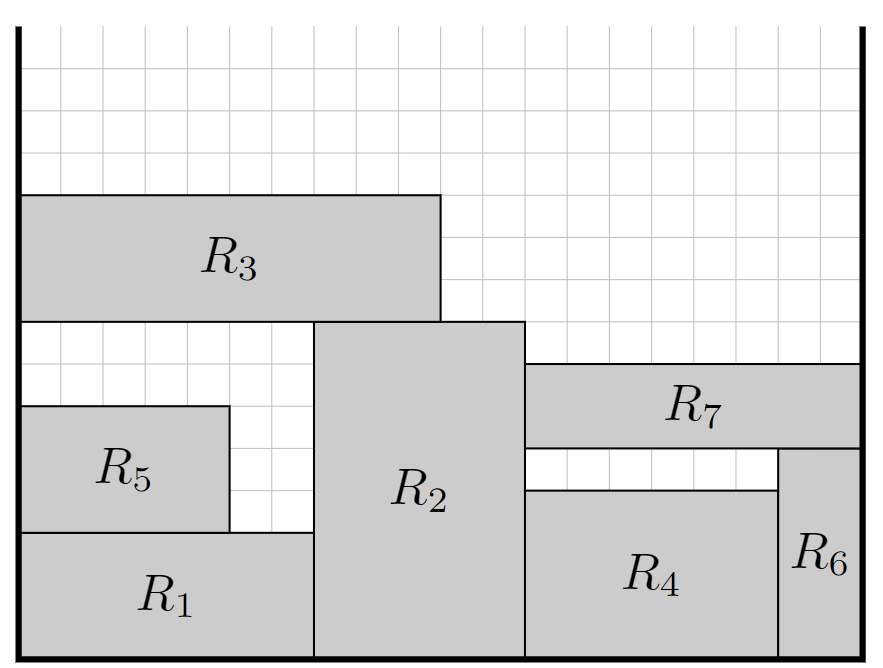
\includegraphics[scale=0.5]{2dpacking}
  \caption{2D Packing Problem}
  \label{fig:2dpacking}
\end{figure}
The problem plays an important role in many fields. An algorithm for packing can be used to pack items into containers in transportation industry. It is also widely applied in allocating main memory efficiently for multi-processor programming. Basically, this problem can be adapted to most resource allocation problems with two dimension constraints.
\par While the description of this problem is rather simple, there is a hidden computation complexity behind this problem. Actually, this problem is NP-Complete\cite{hartmanis1982computers}, which means that there is probably no efficient deterministic algorithm to solve it. It is easy to notice that this problem is a generalized version of the one-dimension bin packing problem\cite{johnson1974worst}. By restricting the height of all rectangles to be 1, this problem degenerates to one-dimensional bin packing problem. We can reduce the one-dimensional bin packing problem to this problem using the idea above. Because the one-dimensional bin packing problem is NP-Hard, this problem is also NP-Hard. Since an optimized solution to the 2D Packing problem can be easily verified, the 2D Packing Problem is also in NP. Combining both above, we derive that 2D Packing Problem is NP-Complete. With $P$ $vs$ $NP$ being an open problem, we cannot find an efficient algorithm for 2D Packing Problem. \par
Another interesting NP-Complete problem related to 2D Packing is MakeSpan \cite{graham1966bounds} where we try to schedule jobs across multiple machines and minimize the total execution time. By simply restricting all the rectangles' height to be 1, 2D Packing Problem becomes the MakeSpan minimization problem. By finding an efficient algorithm for 2D Packing Problem, we can obtain an efficient solution to the MakeSpan minimization problem as well. \par
We already show that 2D Packing Problem is NP-Complete, and P vs NP remains an open problem, for which we probably cannot find an efficient algorithm to solve it deterministically. To solve an inherently difficult problem, various approaches have been well studied. We can use randomized algorithms to give the correct result with high probability for decision problems, while for optimization, we can use another approach: approximation algorithms\cite{garey1976approximation} which could produce a sub-optimal but reasonable result. \par
In this paper, we investigate various approximation algorithms for 2D Packing. In section 2, we briefly study the definition and performance metric for approximation algorithms. In section 3, we introduce two early level-oriented heuristic approximation algorithms\cite{coffman1980performance}. In section 4, we analyze a more advanced approach\cite{steinberg1997strip} which gives a tighter approximation bound. A brief conclusion and future investigation problems are given in section 5.
\section{Approximation Algorithm}
For inherently difficult problems like NP-Complete problems, various approaches have been well-studied to efficiently solve them. The most common approach to solve an optimization problem is by utilizing approximation algorithms. Approximation algorithms aim to find an approximate solution to the optimal solution, with which we can solve the target problem efficiently with a tight performance bound.\par
The analysis for approximation algorithms often requires a thorough mathematical proof for the worst-case performance. We can find some surprising properties for hard problems through approximation. Although all NP-Complete problems are equivalently difficult, their complexity varies from the perspective of approximation algorithms. For example, there exist an algorithm for the Knapsack problem that can produce solutions that are arbitrarily close to the optimal result in polynomial time with respect to input size and precision. However, finding a solution that is constant-bounded to the optimal result for the Maximum clique problem is proved to be equivalent to prove whether P = NP. Therefore, approximation algorithms offer an extra, more fine-grained classification for NP-hard problems.
\subsection{Approximation Ratio}
To measure the performance of approximation, we need to quantify the difference between the produced result and the optimal solution. The most commonly used metric is the multiplicative factor between the solution and the optimum. For problem $L$, assume that the algorithm is $A$, the optimal result is $OPT(L)$, and the produced solution is $A(L)$:
$$R(A) = max(\frac{OPT(L)}{A(L)}, \frac{A(L)}{OPT(L)})$$
Then for minimization problems, approximation ratio $\alpha$ puts a multiplicative maximum bound on the result $A(L) \leq \alpha*OPT(L)$. For maximization problems, approximation ratio puts a multiplicative minimum bound on the result $A(L) \geq \frac{OPT(L)}{\alpha}$. We can also call this ratio Absolute Approximation Ratios to be precise.
\subsection{Asymptotic Approximation Ratio}
Different from Absolute Approximation ratio that only uses a multiplicative bound factor, Asymptotic Approximation uses an additional additive bound factor. This gives us a more fine-grained metric to measure the performance of Approximation algorithms. For minimization problems, the Asymptotic bound is $\alpha$ when
$$ A(L) \leq \alpha*OPT(L) + \gamma $$
where $\gamma$ is an additive constant factor. It should be noticed that any asymptotic approximation ratio can be relaxed into a weaker absolute approximation bound.\par
Now that we have introduced the metrics for measuring performance of approximation algorithms, we will apply these skills on analyzing 2 intuitive approximation algorithms for 2D Packing in the next section.
\section{Early Approximation Algorithm for 2D Packing}
In this section, we are going to look at some 2-dimensional analogs of the one-dimensional approximation packing algorithms\cite{johnson1974worst}-NFDH and FFDH algorithms. NFDH has an asymptotic approximation ratio of 2 and an absolute approximation ratio of 3. FFDH has a tighter asymptotic approximation ratio of 1.7 and a corresponding absolute approximation ratio of 2.7. We are also going to see the proof of these approximation ratios and gain some insight into the analysis for approximation algorithm.\par
Both NFDH (Next-Fit Decreasing-Height) and FFDH (First-Fit Decreasing-Height) algorithms are level-based\ref{fig:level-based}, which means that the packing will be a sequence of levels. Each level is horizontal lines on top of the highest rectangle from the previous level and the first level is simply the bottom of the bin. All the rectangles must place their bottoms on one of these levels. So rectangles can not be placed on top of each other inside each level.
\begin{figure}[htbp]
  \centering
  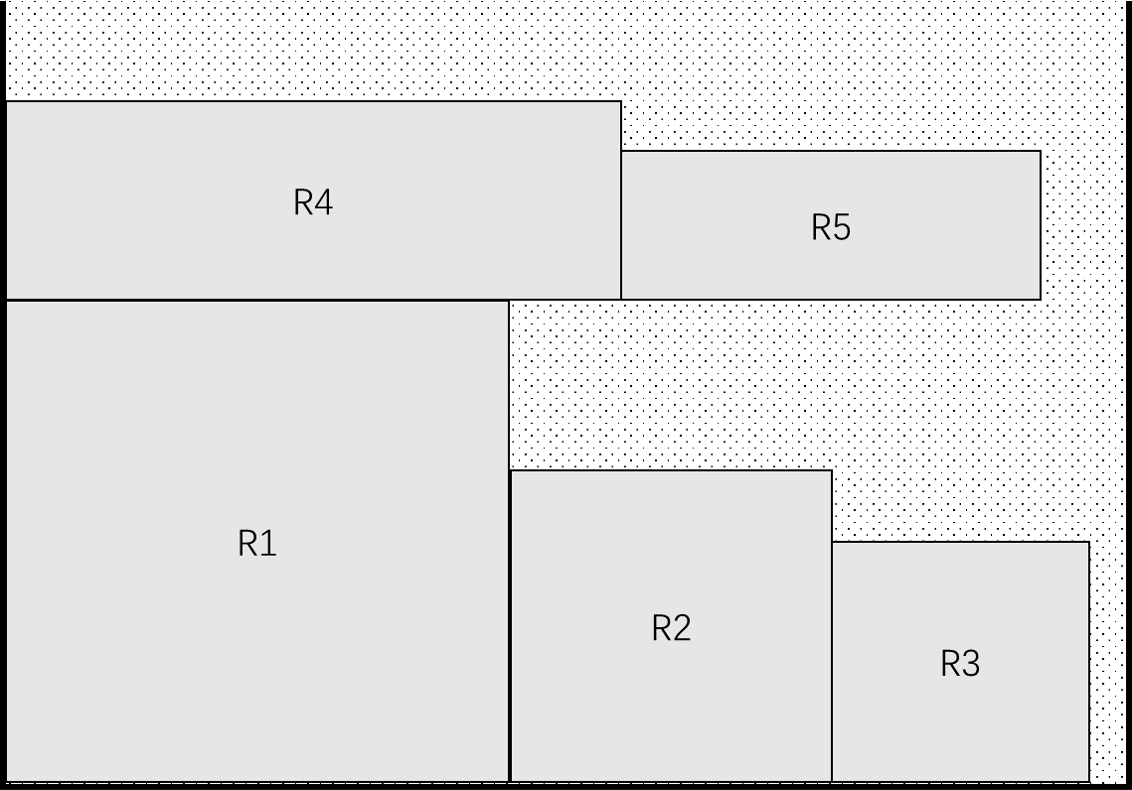
\includegraphics[scale=0.4]{levelbased}
  \caption{Level-Based Packing}
  \label{fig:level-based}
\end{figure}
At first glance, this level-based approach seems wasteful because the space between the level and the rectangle below it is not used. One might think that by putting the rectangle at the lowest-possible place we can achieve a much better result. But as we will show later in the analysis, this new approach will only reduce an additive constant factor which will not affect the algorithm's asymptotic approximation ratio.\par
NFDH and FFDH both are two-dimensional variations of the one-dimensional packing algorithm\cite{johnson1974worst}. They all have a preprocessing procedure to sort all the rectangles with decreasing height. We will introduce both of the 2 algorithms and analyze their approximation ratio in the following subsections.
\subsection{NFDH (Next-Fit Decreasing-Height)}
\paragraph*{Algorithm Description}
NFDH proceeds as follows: After we sort all the rectangles with decreasing height. We simply pack rectangles left-justified from left to right on the bottom of the bin (the first level), so the first rectangle is the highest rectangle. When there is no more sufficient width in the current level, we proceed to the next level (a horizontal line on top of the first rectangle in the current level). We just iterate from level to level until we pack all the rectangles.
\paragraph{Performance Analysis}
It may seem that we are wasting space by using the level-based NFDH algorithm, but NFDH has an asymptotic approximation ratio of 2 with an additive factor $h_{max}$ which is the maximum height of all the rectangles and an absolute approximation ratio of 3.
$$NFDH(L) \leq 2*OPT(L) + h_{max}$$
The analysis is shown below, we are normalizing the bin width to be 1 for simplicity.\par
First, we need to introduce some extra symbols for representation. Assume that $x_i$ is the width of the first rectangle at level $i$, $H_i$ is the height of level $i$, $W_i$ is the total weight of level $i$. Then because the first rectangle of level $i+1$ is too big to fit in level $i$, $W_{i} + x_{i+1} \geq 1$ holds. This inequality is used in the proof to relax the result. $A_i$ is the area of level $i$, and $A$ is the total area of all the rectangles. \par
The main idea of the proof is to find a bounded relationship between $A$ and the result $NFDH(L)$. Because the optimal result $OPT(L)$ has to be bigger than the total area $A$, we are able to find an inequality between $NFDH(L)$ and $OPT(L)$. The detailed proof is as follows:
\begin{align*}
  NFDH(L) = \Sigma_{i=1}^{t}H_i  &\leq H_1 + \Sigma_{i=1}^{t-1}H_{i+1}*(W_i + x_{i+1})\\
                & = H_1 + \Sigma_{i=1}^{t-1}(H_{i+1}*W_i + H_{i+1}*x_{i+1})\\
                & \leq H_1 + \Sigma_{i=1}^{t-1}(A_i + A_{i+1})\\
                & \leq H_1 + 2*A\\
                & \leq H_1 + 2*OPT(L)\\
                & = 2*OPT(L) + h_{max} \\
                & \leq 3*OPT(L)
\end{align*}
We will also provide an intuition into the complicated proof: Measuring the approximation ratio for 2D Packing is equivalent to measure how much space we are wasting during packing. For the NFDH algorithm, the wasted space is the empty space between levels. For each level $i$, we draw a horizontal line of height $H_{i+1}$ (which is $\leq H_i$), then we are able to partition the wasted space into 2 areas $S_i$ (the empty space above the line) and $T_i$ (the empty space below the line). $S_i$ has width at most $1$ and height at most $H_i - H_{i+1}$. Because we are packing rectangles with decreasing height, every rectangles in level $i$ is higher than $H_{i+1}$, therefore every $T_i$ has width $1-W_i$ which is smaller than $x_{i+1}$ according to the inequality $W_{i} + x_{i+1} \geq 1$, $T_i$ has height $H_{i+1}$. Then we know that $S_i \leq 1*(H_i - H_{i+1}) = H_i - H_{i+1}$ and $T_i \leq (1 - W_i)*H_{i+1} \leq x_{i+1}*H_{i+1} \leq A_{i+1}$. Then by summing them up, we get $$S = \sum_{i=1}^{t} S_{i} \leq \sum_{i=1}^{t} (H_i - H_{i+1}) = H_1 - H_t \leq H_1 = h_{max}$$ $$T = \sum_{i=1}^{t}T_i \leq \sum_{i=1}^{t}A_{i+1} \leq A$$
Then we are only wasting $A + h_{max}$ spaces, therefore the result: $$NFDH(L) = A+S+T \leq 2*A + h_{max} \leq 2*OPT(L) + h_{max}$$
It is also worth mentioning that $S$ (the wasted space between the top of rectangles and the level lines) is the total space wasted by using a level-based approach rather than putting every rectangle at the lowest possible position. Because $S \leq h_{max}$, we know that the level-based approach will only introduce a maximum waste of an additive constant and will not affect the asymptotic approximation ratio.
\subsection{FFDH (First-Fit Decreasing-Height)}
\paragraph*{Algorithm Description}
FFDH basically follows the same procedure as NFDH except that now we can also pack rectangles in the previous level to reuse the wasted space. As shown in figure\ref{fig:ffdhpacking}, $R_6$ will be packed in level 3 for NFDH but is packed in level 1 for FFDH to reuse space. This algorithm definitely performs better than NFDH and has a slightly better asymptotic approximation ratio of 1.7 and an absolute approximation ratio of 2.7. However, it should be noted that FFDH will increase memory usage because it has to track the available width for all the previous levels.
\begin{figure}[htbp]
  \centering
  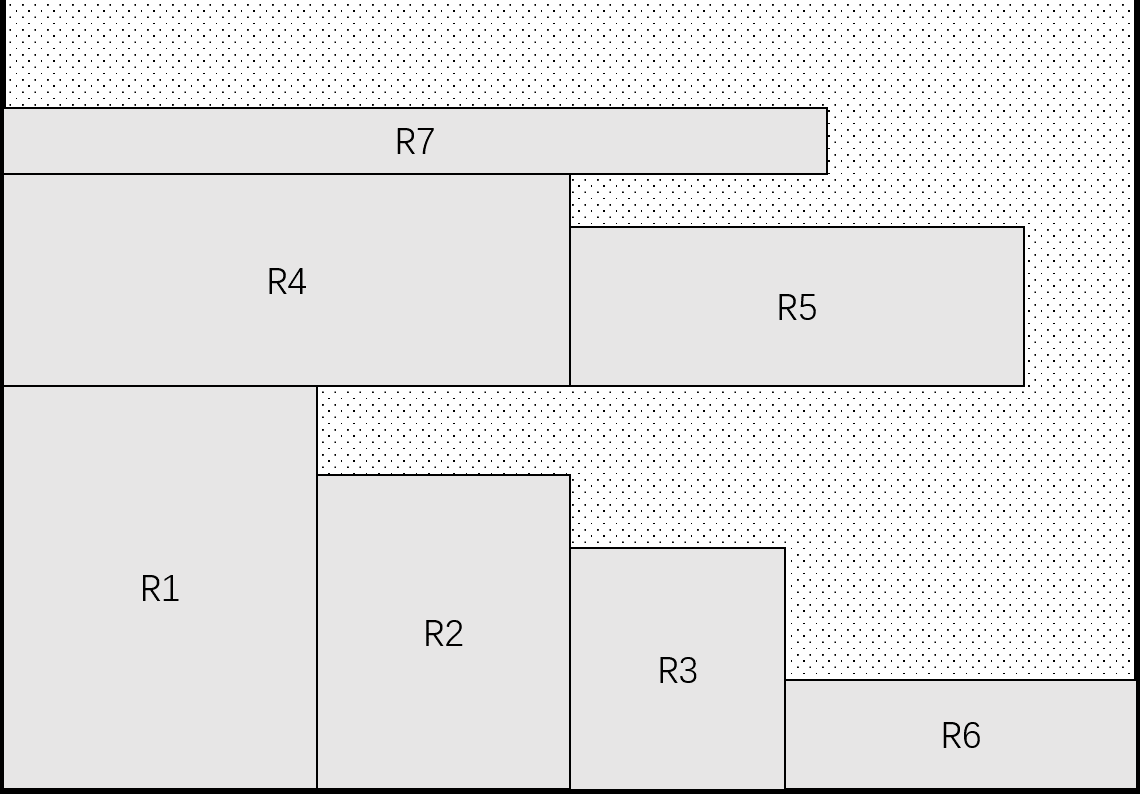
\includegraphics[scale=0.4]{ffdh}
  \caption{FFDH Packing}
  \label{fig:ffdhpacking}
\end{figure}
\paragraph{Performance Analysis}
FFDH has an asymptotic approximation ratio of 1.7 which means that:
$$FFDH(L) \leq 1.7*OPT(L) + h_{max}$$
The main idea of the proof for this approximation ratio is to find an intermediate bound between the total area of rectangles $A$ and $FFDH(L)$. The helper function $W(x)$ used to define the bound in\cite{coffman1980performance} is:
$$ W(x)=\left\{
\begin{aligned}
& \frac{6}{5}x  &   if \text{ } & 0 \leq x \leq \frac{1}{6}\\
& \frac{9}{5}x - \frac{1}{10}  &   if \text{ } & \frac{1}{6} < x \leq \frac{1}{3}\\
& \frac{6}{5}x + \frac{1}{10}  &   if \text{ } & \frac{1}{3} < x \leq \frac{1}{2}\\
& \frac{6}{5}x + \frac{2}{5}  &   if \text{ } & \frac{1}{2} < x \leq 1
\end{aligned}
\right.
$$
And it is shown in\cite{garey1976resource} that no collection of $x$ summing to 1 can have $W(x)$ sum to more than 1.7. Coffman's paper\cite{coffman1980performance} uses this helper function to bound the optimal result by split the optimal solution into pieces\cite{coffman1980performance}. The intermediate bound is as follows:
$$I = \sum_{r \in R}h(r)*W(w(r)) \leq 1.7*OPT(L)$$
The paper also forms an inequality between the result $FFDH(L)$ and $I$:
$$I \geq FFDH(L) - h_{max}$$
The proof for this inequality is very complicated so we will not dig into that in this paper, you can always read the full comprehensive proof in\cite{coffman1980performance}. Then by combining the two inequalities, we can get the relationship between $FFDH(L)$ and $OPT(L)$:
$$FFDH(L) \leq I + h_{max} \leq 1.7*OPT(L) + h_{max} \leq 2.7*OPT(L)$$
Then we can conclude that $FFDH$ has an asymptotic approximation ratio of 1.7 and an absolute approximation ratio of 2.7.\par
Now we have looked at the 2 heuristic intuitive approximation algorithms with an absolute approximation ratio of 3 and 2.7, one may wonder is it possible to get a tighter bound using a different approach? The answer is yes, as we will show in the next section, we can get a much better absolute approximation ratio of 2 using a constraints-driven approach.
\section{Steinberg's Algorithm}
\par In this section we introduce a more advanced approximation algorithm designed by \cite{steinberg1997strip}. Instead of heuristically packing every rectangle and output the height as result, Steinberg gave a more specific bound on the height $\hat{h}$ of the bin, with which a valid packing can be found easily. This is guaranteed by the following theorem.
\paragraph{Steinberg's Theorem} Suppose that $w_M=\max_{1\leq i\leq n}w_i$, $h_M=\max_{1\leq i\leq n}h_i$, $a_i=w_ih_i$, and $A=\sum_{i=1}^{n}$. If the following inequalities hold,
\begin{equation}
	w_M\leq w, h_M\leq h, 2A\leq wh-(2w_M-w)_+(2h_M-h)+ 
	\label{cbase}
\end{equation}
then it is possible to pack the rectangles $R_1, R_2, \ldots, R_n$ into the bin $Q$ of size $w\times h$ by an efficient algorithm $M$\cite{steinberg1997strip}. The plus footnote returns the rectified linear value by $x_+=\max(x,0)$, which is a non-negative term.
\par Intuitively, inequalities \ref{cbase} states that the problem of packing the rectangles would be easy when the total area of $R_1$ to $R_n$ compared to the bin is not too big. This is consistent with our observation that when the bin is fairly large, simply sequentially packing rectangles would suffice.
\paragraph{Steinberg's algorithm for 2D packing} Based on the theorem, Steinberg gave a straight-forward algorithm to answer 2D packing problem. On input $R_1, R_2, \ldots, R_n$, the minimum $\hat{h}$ such that inequalities \ref{cbase} are satisfied with respect to bin $\hat{Q}$ of size $1\times \hat{h}$ is calculated as output. By substitution, the closed form representation of $\hat{h}$ is given by
\begin{equation}
	\hat{h}=\inf\{h:h_M\leq h \wedge 2A\leq h-(2w_M-1)_+(2h_M-h)_+\}
\end{equation}
It is easy to check that
\begin{equation}
	h=\max\{h_M, 2A+(2-\frac{1}{w_M})_+(h_M-A)\}
\end{equation}
which can be further relaxed to
\begin{equation}
	\hat{h}\leq A+\max(h_M, A)\leq OPT(L)+OPT(L)=2OPT(L)
\end{equation}
This gives an absolute performance bound of 2, which is a great improvement from the asymptotic performance bounds by former heuristic methods.
\paragraph{Recursive construction for $M$} Now we turn to the construction for the core algorithm $M$ for the correctness of the algorithm above. Steinberg designed several mutually disjoint reduction procedures that are applied when specific geometric properties are observed in input instances. Specifically, the input is categorized to fall into one of four classes $C_0, C_1, C_2, C_3$, where corresponding procedures $P_0,P_1, P_2,P_3$ would either solve $L$ or reduce to problems of smaller sizes.
\par The four classes are designed as below.\\
(C0) $w_M\leq \frac{w}{2}, h_M\leq\frac{h}{2},$ and for some index $i\in[1,n]$ we have $A-\frac{1}{4}wh\leq a_i$; \\
(C1) $w_M\geq \frac{w}{2}$; \\
(C2) $w_M\leq \frac{w}{2}, h_M\leq\frac{h}{2}$, and there exists two different indices $i$ and $k$ such that $w_i\geq \frac{w}{4}, w_k\geq\frac{w}{4}, h_i\geq\frac{w}{4}, h_k\geq\frac{h}{4}, 2(A-a_i-a_k)\leq (w-\max(w_i, w_k))h$; \\
(C3) $w_M\leq\frac{w}{2}, h_M\leq\frac{h}{2}, n>1$, and for some index $m\in[1,n)$ we have $A-\frac{1}{4}wh\leq\sum_{i=1}^{m}s_i\leq\frac{3}{8}wh$ and $w_{m+1}\leq\frac{w}{4}$. 
\par Since the height and weight components in $C_1$ to $C_3$ play a non-symmetrical role, we can interchange the positions of $w_M$ with $h_M$ and $w$ with $h$ to obtain transposed procedures $P_{-1}, P_{-2}$ and $P_{-3}$ which are applied to transposed classes $C_{-1}, C_{-2}, C_{-3}$, thus allowing for the rotation of input rectangles. It is shown that if input instance $(Q,L)$ satisfies inequalities \ref{cbase}, then it must satisfy one of the conditions $C_\mu$ with $\mu\in[-3,3]$ \cite{steinberg1997strip}.
\par For input instances satisfying C0 apart from inequalities \ref{cbase}, P0 first places rectangle $R_i$ so that $_*[R_i]=_*Q$, where $_*Q$ denotes the left bottom corner of bin $Q$. If $n=1$, then $(Q,L)$ is solved; otherwise, P0 forms a new problem $(Q^\prime, L^\prime)$, where new bin $Q^\prime$ is defined by
\begin{equation}
	_*[Q^\prime]=[R_i]_*, [Q^\prime]^*=Q*
\end{equation}
where $[R_i]_*$ denote the right bottom corner for $R_i$ and $Q^*$ denotes the upper right corner for $Q$. $L^\prime$ is obtained by removing $R_i$ from $L$. The new problem $(Q^\prime, L^\prime)$ can be verified to still satisfy inequalities \ref{cbase}.
\par For input instances satisfying C1, P1 first sort all rectangles by their width and find the maximal index $m$ such that $w_m\geq\frac{w}{2}$ and $w_m<\frac{w}{2}$. The pieces $R_1$ to $R_m$
\begin{figure}[htbp]
	\centering
	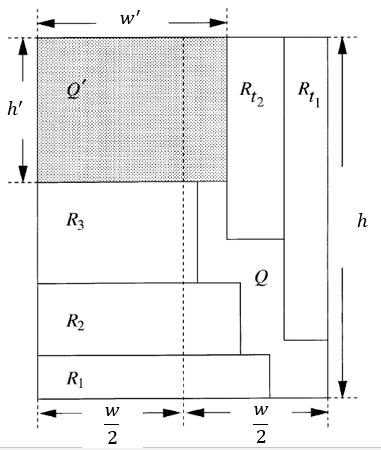
\includegraphics[width=\linewidth]{steinC1}
	\caption{Illustration for packing in Procedure P1}
	\label{steinC1Illus}
\end{figure}
are just placed in the left bottom side with $_*[R_1]=_*Q$ and $_*[R_i]=^*[R_{i-1}]$ for $i\geq 2$. If $m=n$, then input instance is solved. Otherwise, P1 sorts the remaining rectangles by height and place them in the similar symmetric fashion if the largest height in the remaining pieces exceeds the uncovered height $h^\prime$ as shown in Fig. \ref{steinC1Illus}. If not exceeding, then the top region can already constitutes a sub-problem $(Q^\prime, L^\prime)$ with $_*[Q^]=^*[R_m]$ and $[Q^\prime]^*=Q^*$ and $L^\prime=L-\{R_1, R_2, \ldots, R_m\}$, which can be shown to satisfy inequalities \ref{cbase}. If exceeded, then the remaining region and rectangles makes up a new problem, which is also shown to satisfy inequalities \ref{cbase}\cite{steinberg1997strip}.
\par For input instances satisfying C2, P2 places rectangles $R_i$ and $R_k$ at the bottom left so that $_*[R_i]=_*[Q]$ and $_*[R_k]=^*[R_i]$ just like first phase of P1. If $n=2$, then the problem is solved; otherwise, P2 forms a new problem $(Q^\prime, L^\prime)$ where $_*[Q^\prime]=[R_i]_*$, $[Q^\prime]=Q^*$ and $L^\prime=L-\{R_i, R_k\}$.
\par For input instances satisfying C3, P3 cut $Q$ into two rectangles $Q^\prime$ and $Q^{\prime\prime}$ with width $w^\prime$ and $w^{\prime\prime}$ given as follows:
\begin{equation}
	w^\prime=\max(\frac{w}{2},\frac{2Z}{w}), w^{\prime\prime}=\min(\frac{w}{2},w-\frac{2Z}{w})
\end{equation}
where $Z=\sum_{i=1}^{m}a_i$. The two sub-problems are given by $(Q^\prime,L^\prime)$ and $(Q^{\prime\prime},L^{\prime\prime})$, where the height for $Q^\prime$ and $Q^{\prime\prime}$ are still $h$, and $L^\prime=\{R_1,R_2,\ldots,R_m\}$ and $L^\prime\prime=\{R_{m+1},R_{m+2},\ldots, R_n\}$. Both problems are shown to still satisfy inequalities \ref{cbase}.
\par From all the construction for all procedures, we can construct $M$ which on every input instances $(Q,L)$ selects the appropriate Procedure $P_\mu$ and either stop if it is already solved, or applied to the sub-problems it generated. By storing three presorted linked lists corresponding to decreasing order of width, height and area, the placement of rectangles for each phase can be implemented efficiently. By induction, the running time of $M$ is in $O(\frac{n\log^2 n}{\log\log n})$, which is almost linear to input size.
\section{Conclusion}
\par In this paper, we give the formal definition for the problem of 2D packing and analyze the intrinsic difficulty in giving a deterministic solution in polynomial time. We then introduce the common notations and concepts of approximation algorithms to attack this problem. Two early algorithms, NFDH and FFDH which approximates the optimal solution by stacking rectangles heuristically are introduced and their performances bounds are calculated. We finally study a more advanced algorithm on 2D packing which gives a feasible height that allows for efficient solution to packing in the first place. The idea is further used in other works related to higher dimensional packing \cite{approx3okp}.
\par Based on our study so far, we plan to look into the following problems in the future:
\begin{itemize}
	\item (Extraordinary) It has been shown that there exists no polynomial time approximation algorithm for 2D packing with a ratio smaller than $1.5$ unless $P=NP$. People have reached $\frac{5}{3}+\epsilon$ so far. How close to $1.5$ can we achieve on this problem?
	\item (Middle) Approximation algorithms for a natural extension of this problem, 3D packing, generally has a worse approximation ratio than this one. Simply applying NFDH and FFDH techniques can lead to arbitrarily bad approximation ratios. Is there an intrinsic difference in difficulty of packing with respect to dimension? If so, why is it happening? How quick does this difficulty change?
	\item (Short-term) The Steinberg's method actually does not pack the items when giving the prediction. If some packing exercise on input is allowed, can we reach a better bound? If $M$ is allowed more time, can we do any better?
\end{itemize}
\bibliographystyle{acm}
\bibliography{paper}
\end{document}
\endinput
